\documentclass[12pt]{article}
\usepackage[utf8]{inputenc}
\usepackage{graphicx}
\usepackage{enumitem,amssymb}
\usepackage{tabularx}
\usepackage{calc}
\usepackage{cprotect}
\usepackage{xcolor}
\usepackage[a4paper,textwidth=16cm,top=2cm,bottom=2cm,headheight=25pt,headsep=12pt,footskip=25pt]{geometry}
\usepackage{fancybox}
\newenvironment{framed}%
  {\begin{Sbox}\begin{minipage}{\dimexpr\linewidth-2\fboxrule-2\fboxsep}}%
  {\end{minipage}\end{Sbox}\fbox{\TheSbox}}

\usepackage{pifont}
\usepackage{ifthen}

\newcommand{\corrige}{0}
\newcounter{possibility}\newcommand{\correct}{%
  \addtocounter{possibility}{1}
  \ifthenelse{\equal{\corrige}{0}}%
    {\item[\textcolor{red}{\ding{\numexpr171+\value{possibility}}}]}%
    {\item[\ding{\numexpr171+\value{possibility}}]}%
}

\newcommand{\leurre}{%
  \addtocounter{possibility}{1}
  \item[\ding{\numexpr171+\value{possibility}}]%
}

\newcommand{\enonce}[1]{%
  \noindent
  Question~:
  \vspace*{.5\baselineskip}

  \noindent
  \begin{framed}
    #1
  \end{framed}
}

\newcommand{\difficulte}[1]{%
  Difficulté : 
  \ifthenelse{#1 > 1 \or #1 = 1}{\ding{72}}{\ding{73}} 
  \ifthenelse{#1 > 2 \or #1 = 2}{\ding{72}}{\ding{73}}
  \ifthenelse{#1 > 3 \or #1 = 3}{\ding{72}}{\ding{73}}
  \ifthenelse{#1 > 3}{S}{}%
}

\newcommand{\possibilites}[1]{%
  \setcounter{possibility}{0}
  \vspace*{\baselineskip}
  \begin{itemize}[label={}]
    #1
  \end{itemize}
}


\newcommand{\pourquoi}[1]{}

\begin{document}
\begin{center}
  \begin{tabular}{c}
  \hline\\%\vspace{0.1cm}
  {\textsc{\'Ecole Centrale Marseille}}\vspace{0.1cm}
  \\

    {\bf {\Large Modélisation et Conception Objet}}\\%\vspace{0.2cm}
    \\
    {\bf  { Contrôle 1A }}\\
    {\footnotesize 05/06/2025}\\
    \hline
  \end{tabular}
\end{center}
\vspace{0.6cm}

\noindent
{\em Les réponses sont à donner directement sur le sujet. Un espace est réservé pour chaque réponse.}

\vspace*{1cm}
\noindent
\begin{tabular}{|l|p{10cm}|}
    \hline
    Nom : & \\
    \hline
    Prénom : & \\
    \hline
    
\end{tabular}


\vspace*{2cm}
\noindent
Barème. Pour chaque question : 
\begin{itemize}
    \item ne pas répondre donne 0 point,
    \item répondre de façon exacte donne : $\mathbf{+\frac{2}{3}}$ points
    \item répondre de façon inexacte\footnote{le nombre de points négatifs varie pour que si l'on répond de façon aléatoire l'espérance soit nulle} : 
    \begin{itemize}
        \item pour une réponse de type VRAI/FAUX : $\mathbf{-\frac{2}{3}}$ points,
        \item pour une réponse libre : $\mathbf{-\frac{2}{3}}$ points,
        \item pour une réponse de type 1 parmi 3 : $\mathbf{-\frac{1}{3}}$ points.
    \end{itemize}
\end{itemize}
\newpage
\section{}[h]
\difficulte{1}

\enonce{Qui est le plus important entre le main, les tests et les fonctions?}
\setcounter{possibility}{0}
\possibilites{
    \correct \textcolor{red}{Le main}
    \correct \textcolor{red}{Les tests}
    \correct \textcolor{red}{Les fonctions}
}
\pourquoi{}

\begin{figure}[h]
\centering
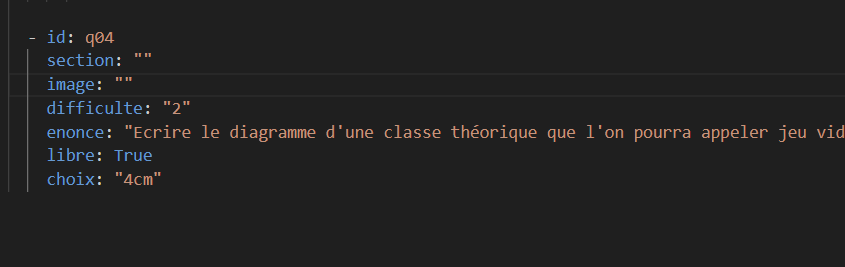
\includegraphics[width=\paperwidth]{image.png}
\end{figure}

\section{}
\difficulte{2}

\enonce{Ecrire le diagramme d'une classe théorique que l'on pourra appeler jeu video donner des attribut et methode en accord avec le nom de cette classe}

\noindent
\begin{tabular}{|p{\dimexpr\textwidth-2\tabcolsep-2\arrayrulewidth}|}
\hline
\parbox[t][4cm][c]{\dimexpr\textwidth-2\tabcolsep-2\arrayrulewidth}{}
\\
\hline
\end{tabular}


\end{document}